%\documentclass[twocolumn]{article}
\documentclass[12pt]{article}
% Change "article" to "report" to get rid of page number on title page
\usepackage{amsmath,amsfonts,amsthm,amssymb}
\usepackage{setspace}
\usepackage{fancyhdr}
\usepackage{lastpage}
\usepackage{extramarks}
\usepackage{chngpage}
\usepackage{soul}
\usepackage[usenames,dvipsnames]{color}
\usepackage{graphicx,float,wrapfig}
\usepackage{listings}
\usepackage{framed}
\usepackage{inconsolata}
\usepackage{cite}

% Stuff to change, you know, if you want.
\setlength{\parindent}{1cm}
\setlength{\parskip}{3pt}

% In case you need to adjust margins:
\topmargin=-0.45in      %
\evensidemargin=0in     %
\oddsidemargin=0in      %
\textwidth=6.5in        %
\textheight=9.0in       %
\headsep=0.25in         %

\pagestyle{empty}

\newcommand{\framedscalefigone}[3]{
  \begin{figure}[ht!]
    % Requires \usepackage{graphicx}
    \centering
    \begin{framed}
      \begin{minipage}{\textwidth}
        \centering
        \includegraphics[width=#2\columnwidth]{#1}
        \caption{#3}
        \label{#1}
      \end{minipage}
    \end{framed}
  \end{figure}}

\newcommand{\framedscalefigtwo}[4]{
  \begin{figure}[ht!]
    % Requires \usepackage{graphicx}
    \centering
    \begin{framed}
      \begin{minipage}{0.49\textwidth}
        \includegraphics[width=#3\columnwidth]{#1}
      \end{minipage}
      \begin{minipage}{0.49\textwidth}
        \includegraphics[width=#3\columnwidth]{#2}
      \end{minipage}
      \caption{#4}
      \label{#1}
    \end{framed}
  \end{figure}}

\newcommand{\scalefigone}[3]{
  \begin{figure}[ht!]
    % Requires \usepackage{graphicx}
    \centering
    \includegraphics[width=#2\columnwidth]{#1}
    \caption{#3}
    \label{#1}
  \end{figure}}

\newcommand{\scalefigtwo}[4]{
  \begin{figure}[ht!]
    % Requires \usepackage{graphicx}
    \centering
    \includegraphics[width=#3\columnwidth]{#1}
    \includegraphics[width=#3\columnwidth]{#2}
    \caption{#4}
    \label{#1}
  \end{figure}}

\setlength\fboxrule{1pt}

\graphicspath{{../figures/}}

%%%%%%%%%%%%%%%%%%%%%%%%%%%%%%%%%%%%%%%%%%%%%%%%%%%%%%%%%%%%%
% Make title
\title{}
\date{}
\author{}
%%%%%%%%%%%%%%%%%%%%%%%%%%%%%%%%%%%%%%%%%%%%%%%%%%%%%%%%%%%%%
\begin{document}

\begin{center} \begin{Large}
  \textbf{A spiking neural circuit model of cortical function
          in simple reaction time tasks}
\end{Large} \end{center}

\begin{center}
  Trevor Bekolay, Benjamine Liu, Nandakumar Narayanan, Chris
  Eliasmith, Mark Laubach
\end{center}

\begin{abstract}
  todo
\end{abstract}

\section{Introduction}

Animals make complicated motor actions
with high spatial and temporal resolutions.
In temporally precise tasks,
the motor cortex and several afferents coordinate
to bring about motor actions at appropriate times.
For tasks with delay periods,
the medial prefrontal cortex is critically important
for suppressing motor action during the delay period.
This effect has been seen in ?.  %???primates humans rodents etc???.

In rodents, the role of the medial prefrontal cortex
has been investigated through ?.
%???previous work???.
Previously, we have used a simple reaction task
and principal component analysis
to investigate ?. %???summarize Narayana \& laubach jnp 2009???
These results point to neural integration
as playing a key role
in the mPFC's ability
to control the timing of motor actions.

In order to investigate the neural circuit
underlying the production and suppression of motor output,
we extend Singh \& Eliasmith's model to include
neural populations that directly affect the environment,
analogous to the function of Betz cells.
In doing so, we can relate the model to the experimental data
in both neural and behavioural contexts.

\section{Model}

The model presented in this study
is based on a conceptual model of PFC and MC
function in delay tasks proposed by Narayanan and Laubach.
Their conceptual model is based on
principal component analysis of neural data
in rats performing a simple reaction time task.

Figure 1 summarizes their PC analysis.
In PFC, two components account for over 35\%
of variance in population firing.
The first principal component increases slightly
at the time of the lever press,
and then decreases over the delay period.
The second principal component
also increases at the time of lever press,
but remains high until the time of release.

In motor cortex, three components account
for over 60\% of variance in population firing.
The first two principal components are
similar to those found in PFC;
the first steadily decreases over the delay period,
and the second remains high during the delay period.
The third principal component increases
sharply slightly before lever press
and lever release.

The identification of these principal components
leads to a conceptual model of cortical function
during simple reaction time tasks.
This model is summarized in figure 2. % Fig
At the start of a trial,
two complementary systems are activated
to produce quick reactions at the time of a stimulus.
The \textit{prepotent response} system
prepares the motor action that the subject will perform
at the end of the delay period.
The \textit{proactive inhibition} system
suppresses that motor action until the delay period
is over.

\subsection{Neural integration as a core mechanism}

An important observation of Narayanan and Laubach
is that the second principal component
is the cumulative sum (integral)
of the first principal component.
This suggests that some neurons in these cortical areas
are representing the integral of another
signal represented in these areas.

Neural integration through recurrently connected
populations of neurons has been widely studied
in the context of working memory.
% ? cite a bunch -- Mawkinson, Roman, Tanji, X-J Wang, look at singh eliasmith biblio

The Singh and Eliasmith model, in particular,
facilitates a neural implementation of the conceptual model
proposed as a result of the PC analysis.
In addition to outlining a method of constructing
multidimensional neural integrators,
it also provides a method of connecting those integrators
to other populations of neuron representing other signals.

\subsection{Coupled integrators in a control system}

With non-integrative and integrative neuronal populations
as the building blocks, we propose a neural circuit
realization of the conceptual model
discussed in Narayanan and Laubach.
The model is summarized in figure 3.

Two populations are hypothesized to reside in motor cortex.
The \textit{Press/Release} population represents
whether the subject is currently executing
a press or release motor action.
The activity of this population directly affects the environment
in the model, which can be thought of
as functioning like Betz cells.
The \textit{Holding} population tracks
whether or not the subject is currently holding down the lever.
It is analogous to the \textit{prepotent response}
from the conceptual model, as in the absence of inhibition,
it will activate the \textit{Release} neurons
in the \textit{Press/Release} population.
The \textit{Holding} population is integrative,
and integrates the
\textit{Press} signal from the \textit{Press/Release}
population. The integration is controlled
by the \textit{Release} signal, meaning that
when the lever is released the \textit{Holding} signal
is reset to some baseline.

Three populations are hypothesized to reside
in medial prefrontal cortex.
The \textit{Waiting} population represents
that the subject is in a delay state,
waiting for the appropriate time to perform a motor action.
It is analogous to the \textit{proactive inhibition}
from the conceptual model, as it works to balance
the prepotent release response being signaled
from the motor cortex's \textit{Holding} population.
The \textit{Cue} population is sensitive
to the auditory stimulus delivered to the subject
when the delay period is over.
It inhibits the \textit{Waiting} population's
proactive inhibition, disinhibiting \textit{Release}
sensitive neurons.
Similarly, the \textit{Timer} population
tracks the relative amount of time that has passed
since the subject pressed down the lever,
starting the trial.
When the time of the stimulus can be predicted,
the \textit{Timer} population speeds
responding by increasingly inhibiting the
\textit{Waiting} population over time.
It can also effect a motor action on its own by
disinhibiting \textit{Release} neurons sufficiently.
The \textit{Timer} population is integrative,
gradually ramping up as it integrates
the \textit{Waiting} signal.

\section{Methods}

\subsection{Simple reaction time task}

In both the empirical and simulated data,
subjects and models performed the same simple reaction time task.
At the start of a trial,
subjects press down a lever.
A timer tracks the time since the lever was pressed down,
and after an experimenter-specified time period,
called the \textit{delay period} or \textit{foreperiod},
an auditory cue signals that the subject must respond
by releasing the lever.
If the lever is released within 600 milliseconds,
the trial is considered a success
and reward is delivered.
If the lever is released before the auditory cue
or after the 600 millisecond response window,
then the trials is considered a failure
and subjects are given a time out in which
lights are extinguished.
Lever presses during this timeout period
lengthen the timeout period.

Empirically, this study is done with rats
in a MedPC box containing a lever,
house lights, and a spout for delivering water reward.
Rats were trained by first
associating reward with lever presses,
and then introducing progressively longer
delay periods until they reached the goal delay
of 1 second.
They were considered to have learned the task
when they performed the task correctly $>60\%$
of the time.

Theoretically, this study was performed
in the Nengo simulation environment.
Subjects were networks of leaky integrate-and-fire
neurons, as described below.
The environment was modeled using a
\texttt{simplenode}, which allow arbitrary code
to interact with a neural model.
In this case, the \texttt{simplenode} implemented
a finite state machine to track task state,
and scalar values to indicate the state of
house lights, lever position, auditory cue, and reward.

\subsection{Empirical summary}

The empirical study (described in more depth in ?) %???cite???)
was done with twelve male Long-Evans rats (3-4 months old; Harlan).
Rats were water restricted, with food always available,
and consumed 10-15 ml of water during each
behavioural session.

Arrays of recording electrodes were implanted
in dmPFC ($n = 8$), motor cortex ($n = 3$), or both ($n = 1$).
Electrodes were 50 $\mu$m stainless steel wires
with 250 $\mu$m between wires.
Arrays were in configurations of
4 $\times$ 4 or 3 $\times$ 3 $\times$ 2.
Microwire arrays were targeted at dmPFC
based on the following coordinates from bregma:
anteroposterior [AP]: $+$3.2mm;
mediolateral [ML]: $\pm$1.4mm;
dorsoventral [DV]: $-$3.6mm at 10$^\circ$ in the frontal plane.
Motor cortex was targeted with
AP: $-$0.5mm; ML: $\pm$2.5-3.5mm;
DV: $-$1.5mm at $-25^\circ$ in the frontal plane.
Histology was performed to confirm electrode locations
(???see fig???).

Ensemble recordings were done using a
Many Neuron Acquisition Program (Plexon, Dallas, TX).
Spike sorting using principal component analysis (PCA)
and waveform shape identified 414 single units
whose spikes were included in this study.

\subsection{Theoretical}

Two models were created to explain neural processing
in the simple reaction time task.
The first is a double-integrator model,
as is described in ?, %???cite singh eliasmith???,
which allows for precise comparisons
between the spiking behaviour of
the model and the empirical subjects
given a controllable behavioural outcome.
The second is an integrated model that
expands the double-integrator model
to include populations that manipulate the environment,
allowing for the comparison between
the model and empirical behaviour.

Both models are made up of heterogeneous populations
of leaky integrate-and-fire neurons
created and connected using the methods
of Eliasmith and Anderson ?. % ???cite???.
Connections between populations of neurons
are determined based on the function computed
through the connection.
Connection weights are determined
by solving a least-squares minimization
of the function representation
given the tuning properties
of the neurons representing the function parameters,
as described in ? %???singheliasmith???
and in detail in ?. %???eliasmith anderson ???.

\subsubsection{Double-integrator model}

In  %???cite???
it is shown that
a population of heterogeneous adaptive leaky integrate-and-fire neurons
representing a two-dimensional signal
can capture the dynamics of
working memory cells in prefrontal cortex.
There are, however, several network configurations
that can result in a population of neurons
representing two integrated signals,
as shown in figure ?. %???copy fig 5 from paper???.

We adopt the coupled one-dimensional integrator model,
despite little evidence that reciprocal projections
are localized to smaller integrative populations.
Instead, it is the PCA of mPFC activity
that suggests many neurons are
only sensitive to one of the principal components.
Additionally, it is more intuitive
to connect each principal component with
a separate neural population.
The important task, then,
is to connect each population
with the appropriate value being encoded.

Figure ? %???put in???
summarizes our mapping.
The two coupled one-dimensional oscillators represent
the subject's existence in a particular behavioural state
and how long the subject has been in that state.
The behavioural state is entered
once the subject presses down the lever,
modeled by the activation
of a population of press-sensitive neurons.
The timing integrator is driven
by the state population, as follows from ?. %???citesingh???.
Both coupled integrators are controllable
through a second dimension, %(???cite eliasmith here? ???),
which allows the integrators to be
reset to an initial point (0.0)
when reward is delivered to the subject.
The two one-dimensional integrators
are then projected to an output population that
tracks both signals.

The press- and reward-sensitive populations
drive the rest of the activity of the network.
These two populations are driven by the experimenter,
based on the behaviour being simulated.
For example, for a sequence of correct trials,
the press-sensitive population
will be driven strongly at the start of a trial,
followed 1.6 seconds later
by strongly driving the reward-sensitive population.
For error trials, the reward population
is not driven between activations of the press population.

\subsubsection{Integrated motor-mPFC model}

In order to expand the double-integrator model
to directly manipulate elements of the environment,
three additional variables must be accounted for:
release, auditory cue, and control.

The PCA in ? %???kumar???
revealed
neurons that are sensitive to both press and release.
For this reason, the press-sensitive population
was increased in dimensionality
such that the population was sensitive
to both press and release,
in the same manner to the multidimensional
methods used in ?. %???singh eliasmith???.

The auditory cue ?
%??? todo : see if it's necessary to be an integrator ???

Control is the signal
that causes release-sensitive neurons to fire,
resulting in the release of the lever.
Determining how to implement this control
is one of the primary goals
of mPFC research in tasks with delays.
Its implementation is in itself
a hypothesis of how the mPFC and motor cortex interact
in order to perform these tasks.

\subsubsection{Implementing release control}

? %???kumar???
use their PCA to propose a conceptual model,
shown in Fig ?. %???include???.
We extend this model
by associating prepotent response and proactive inhibition
with neural populations and
showing how they can be connected
such that the model can respond
within the 600 ms response window.

In the double integrator model,
a population of neurons tracks the current behavioural state.
In the integrated model, two populations
track a similar but subtly different quantity.
One population is assumed to exist
in motor cortex, and tracks whether or not
the subject is currently holding down the lever.
This is an integrative population,
which is driven by press-sensitive neurons.
The other population is assumed to exist
in medial PFC, and tracks whether or not
the subject should be delaying the release response.
It is primarily driven by the motor cortex's
holding population.

The motor cortex's holding population
sends excitatory projections
to the release-sensitive neurons,
effecting the prepotent response from the conceptual model.
The medial PFC's waiting population
send inhibitory projects
to the release-sensitive neurons,
effecting the proactive inhibition from the conceptual model.
It should be noted that this organization
produces a slight delay between these two quantities,
with prepotent response occurring first,
quickly followed by proactive inhibition.
This is consistent with ?. %???figure from JNP2009???.

The medial PFC's waiting population's activity
is further modulated by two task-related populations.
One is a ramping population that tracks
the time since the press was initiated.
The other is a cue-sensitive population
that is driven by the onset of the auditory cue.
These two populations
release the proactive inhibition,
causing the release neurons to be disinhibited,
effecting the release of the lever.

As will be discussed further in ?, %???sec???,
the similarity between the two populations
may explain why the first two principal components
of motor cortex and mPFC are very similar.

\subsubsection{Model manipulations}

The model is manipulated in three ways
in this study.

The model emulates the effects of aging
by decreasing the number of neurons
in each neural population,
by uniformly decreasing the strength
of each synapse in the network,
and by randomly removing a fraction
of all synapses in the network.

Lesion studies are emulated
by targeted ablations of either
neurons or synapses in or between specific
neural populations.

Cooling is emulated by
lowering the distribution
of neural gains associated with the
leaky integrate-and-fire neurons
in the neural populations being cooled.
Time constants affecting transmission speed
between populations are raised
to emulate slowed transmission speed
as a result of the cooling of white matter.

\subsection{Analysis}

Both empirical and theoretical experiments
produce data in the form of spike trains
and event timestamps.
The files produced by NeuroExplorer and Nengo
were read by a customized version of Neo,
a Python package for reading neurophysiology data files.
The subsequent analysis was done
with custom written scripts in Python
using the NumPy and SciPy libraries for numerical analysis
and Matplotlib for plotting.
All analysis scripts are freely available
at ?. % github URL

\subsubsection{Behaviour}

Figure 4 summarizes a single trial
of the reaction time task.
In both the empirical and theoretical studies,
the following relevant event times are recorded:
lever press, lever release, reward delivery,
trigger stimulus onset, and house light extinguishing.
Sequences of event times can be used to
identify the result of each trial,
as shown in Figure ?.
Filtering the set of event timestamps
for these sequences identifies each trial outcome.

Reaction time distributions are also analyzed
for correct trials.
Reaction time is defined as the difference between
trigger stimulus onset and lever release.

\subsubsection{Neural}

Principal component analysis (PCA)
is used to identify the important features
in spike trains around certain events.
The previously mentioned techniques
were used to isolate an event of interest.
For each neuron, spike trains from 1 second prior to
2 seconds after each instance of an event are isolated.
Each perievent spike train is binned in 1 ms bins and is then
convolved with a Gaussian filter ($\sigma = $ 25 ms;
PCs are consistent with many other $\sigma$ values).
The spike trains were slightly extended
in order to eliminated edge artifacts.
These spike density functions
are normalized to z-scores,
and then averaged over all trials to
produce a matrix in which each row
the normalized average response of a neuron
over the perievent epoch.
PCA was performed on that matrix
using singular value decomposition.
The resulting principal components
were also normalized to z-scores.
The amount of variance accounted for by each principal component
is computed as the square of the component's eigenvalue
over the sum of all squared eigenvalues
(i.e., $s_i^2 / \sum s^2$).

In all analyses, neurons not significantly modulated
during the perievent epoch were omitted.
Specifically, we omitted neurons with average firing rates
under 1 Hz and whose firing rates were non-stationary
across trials
(determined by a Wald-Wolfowitz runs test with $|Z| > 4$).

\section{Results}

\subsection{Model behaviour is less variable}

A stereotypical trial for both the model
and experimental subjects is shown
in Figure 5.
The experimental session lasted ? seconds,
over which ? trials were performed.
? trials were identified as correct trials;
? were premature responses,
and ? were delayed responses.
The model session lasted 500 seconds,
over which ? trials were performed.
? trials were identified as correct trials,
? were premature responses
and ? were delayed responses.

Over all trials for all subjects,
experimental subjects performed ? trials
with a ? \% success rate.
The model performed ? trials with a
? \% success rate.

The distribution of reactions times, shown in figure 5,
is Gaussian-like with a long tail greater than the mean
for both model and data.
The mean reaction time for all experimental subjects
was ? $\pm$ ?.
The mean reaction time for all model subjects
was ? $\pm$ ?.

\subsection{Model principal components are similar}

Principal component analysis on the spike trains
produced by the model show the same number
of primary principal components, with similar shapes.

In the neural populations hypothesized
to reside in motor cortex, as shown in Figure 6,
three leading components are identified.
As in the experimental data,
PC1 is rises around the time of the press
and maintains a high value until the release,
at which point it drops.
PC2, which is very similar
to the cumulative sum of PC1,
is modulated at the time of lever press,
and slowly changes during the delay period.
PC3 is strongly modulated at both the
time of lever press and release.
Firing rates in the model match those in
the data, increasing before the press
and after release.

In the neural populations hypothesized
to reside in medial prefrontal cortex,
as shown in figure 7,
two leading components are identified.
The first component is strongly modulated
around the time of lever press,
and slowly decreases during the delay period.
The second component,
which is similar to the cumulative sum of
PC1, increases at the time of lever press,
and remains high during the delay period.

\subsection{Model manipulations}

Aging results, figure 8.

Lesion results, figure 9.

Cooling results, figure 10.

\section{Discussion}

\subsection{Model behavioural variability is low}

The primary difference is in the amount
of inter-trial and intra-trial variability.
Experimental subjects had several blocks of time
in which they performed as many trials as the model,
but those blocks of time were interrupted by
error trials and time in which the animal
was performing other actions such as grooming.
Within the trial, reaction time distribution
for the model and experimental subjects are
similar but with far less variability.
The model's reactions times
are within the experimental subjects'
mean and standard deviation, however,
suggesting that the model
could have the same variability
by simply injecting noise into the system.
This would also result in
the error trials that are missing in the model.

A better basis for comparison for the model
would be human performance in a similar
reaction time task. ?find some % Look up some behavioural data

\subsection{Model principal components match the data}

While it may be unsurprising
due to the model being inspired by the original
principal component analysis,
it is strong validation for the original conceptual model
that the implemented model maintain
the same principal components
while still being able to simulate behaviours.

? List differences and investigate (with final version of model)

\subsection{Model predictions}

The model manipulations assert that blah has the effect of blah.

Prior studies (some unpublished) have suggested that these are indeed the effects of those things.

Cooling has not been studied in an experimental setting,
and so we take the results as a prediction of the model.

\clearpage

\appendix

\section{Figures}

\begin{figure}
  \centering
    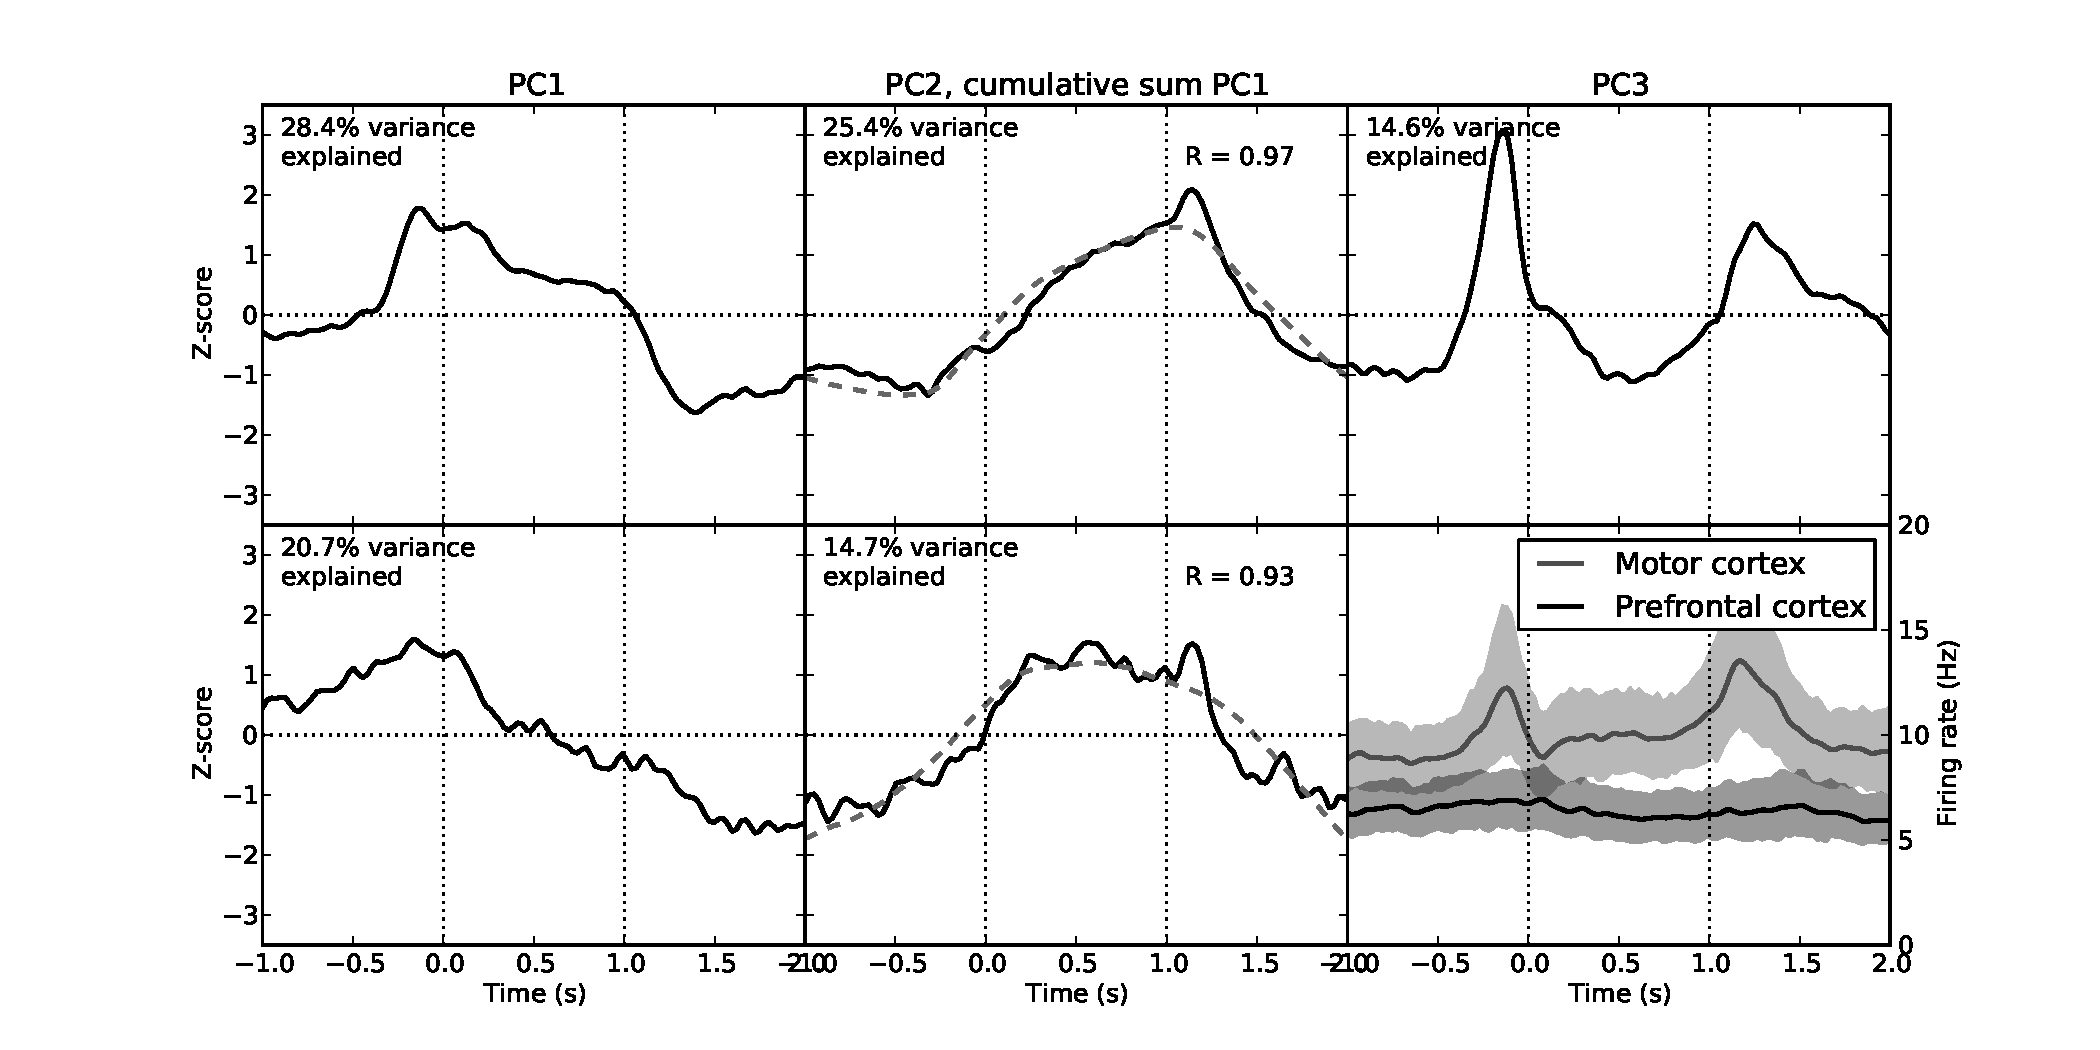
\includegraphics[width=\columnwidth]{f1-pcasummary}
    \caption{Summary of principal components identified
      by Narayanan and Laubach, 2009. Three components
      were identified in motor cortex (top row), accounting
      for over 60\% of variation.
      Two components were identified in prefrontal cortex
      (bottom row), accounting for over 25\% of variation.}
\end{figure}

\clearpage

\begin{figure}
  \centering
    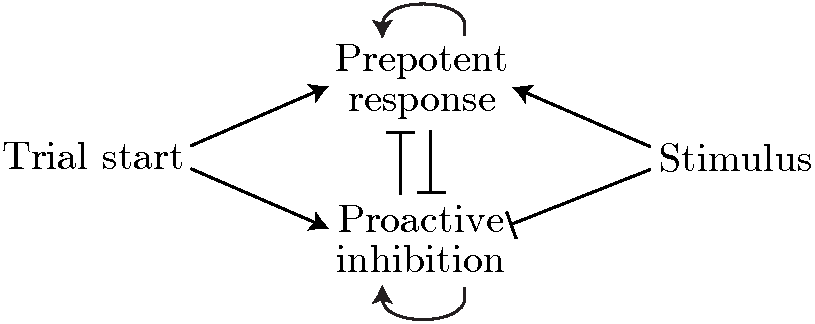
\includegraphics[width=\columnwidth]{f2-conceptual}
    \caption{The conceptual model proposed by Narayana and
      Laubach, 2009. In the conceptual model, the start of the
      trial activates two systems; one prepares the response
      action (prepotent response) and the other inhibits
      that action until the appropriate time (proactive inhibition).}
\end{figure}

\clearpage

\begin{figure}
  \centering
    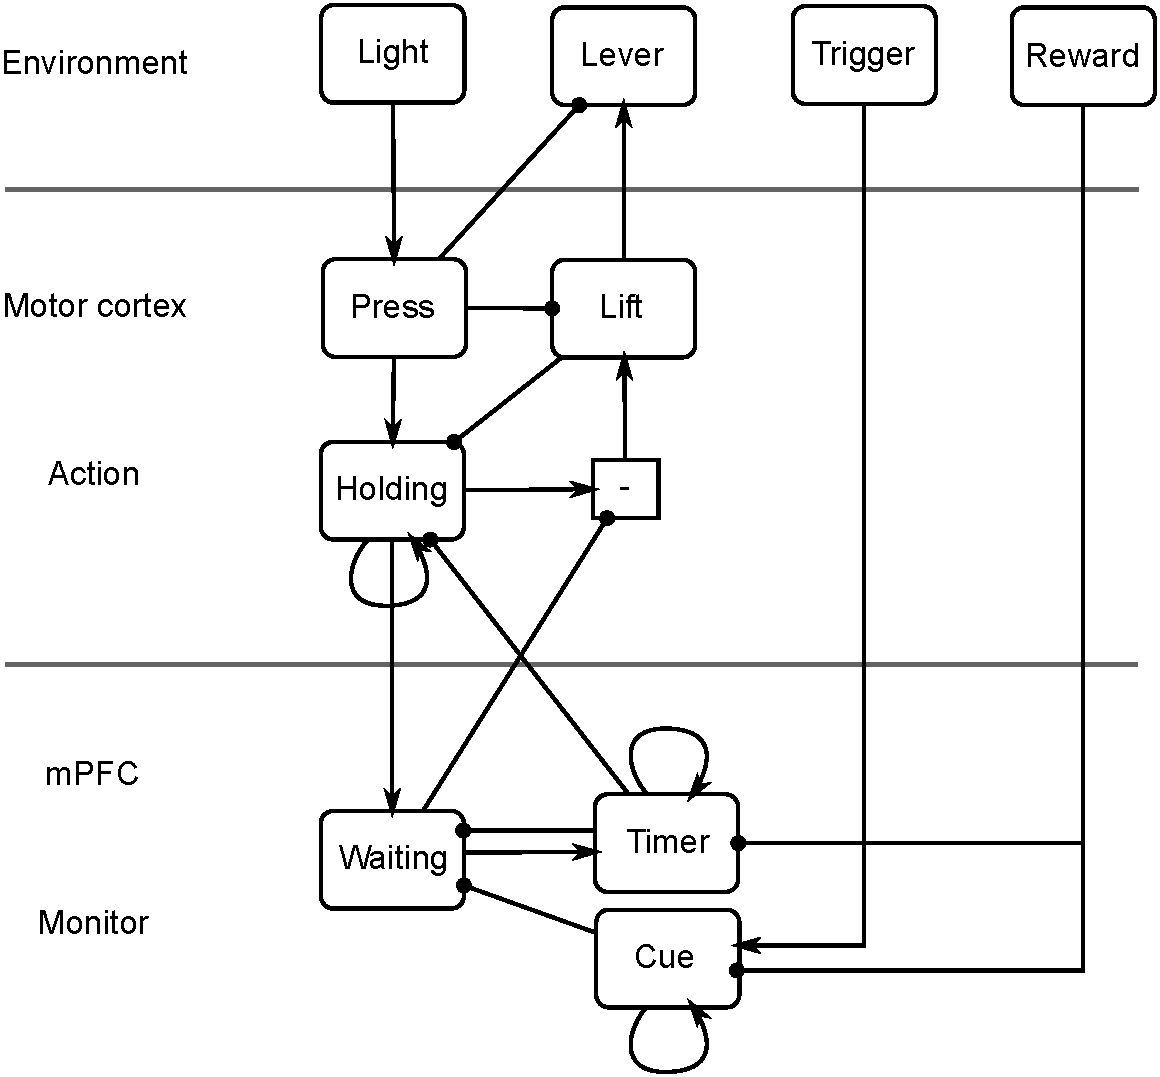
\includegraphics[width=\columnwidth]{f3-fullmodel}
    \caption{The proposed implementation of the conceptual model.
      The motor cortex is made up of two populations of
      leaky integrate-and-fire neurons, one of which interacts
      with the environment by pressing or releasing a lever.
      The medial prefrontal cortex is made up of three
      populations of LIF neurons. See text (section 2) for details.}
\end{figure}

\clearpage

\begin{figure}
  \centering
    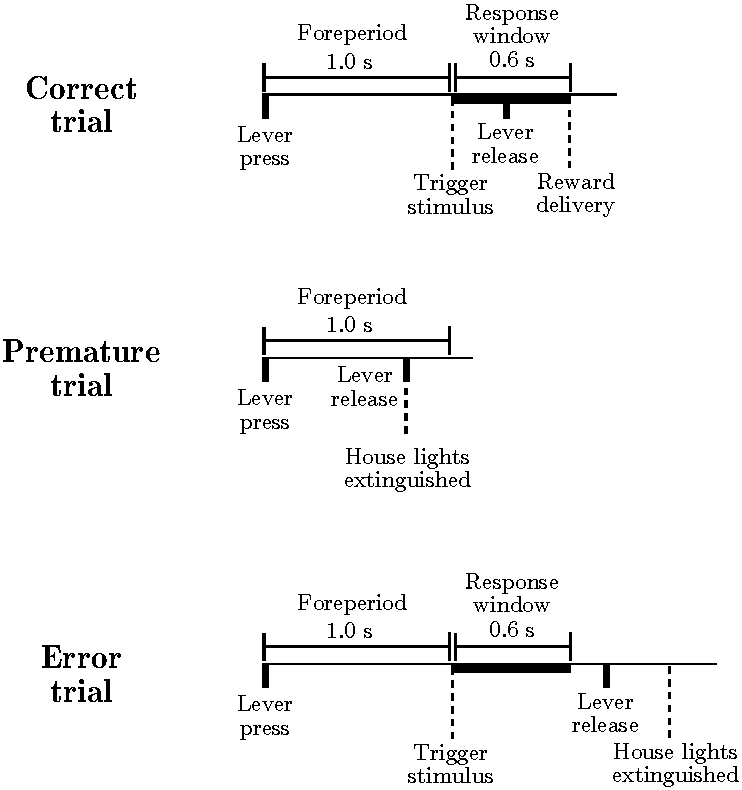
\includegraphics[width=\columnwidth]{f4-behaviour}
    \caption{Possible outcomes for each trial. If the subject
      responds within the 0.6 second response window, the trial
      is counted as correct and reward is delivered. If the
      subject responds prematurely, it is counted as an error
      and house lights are extinguished for a timeout period.
      If the subject responds after the response window,
      an error is also recorded and the lights are extinguished.}
\end{figure}

\clearpage

\begin{figure}
  \centering
    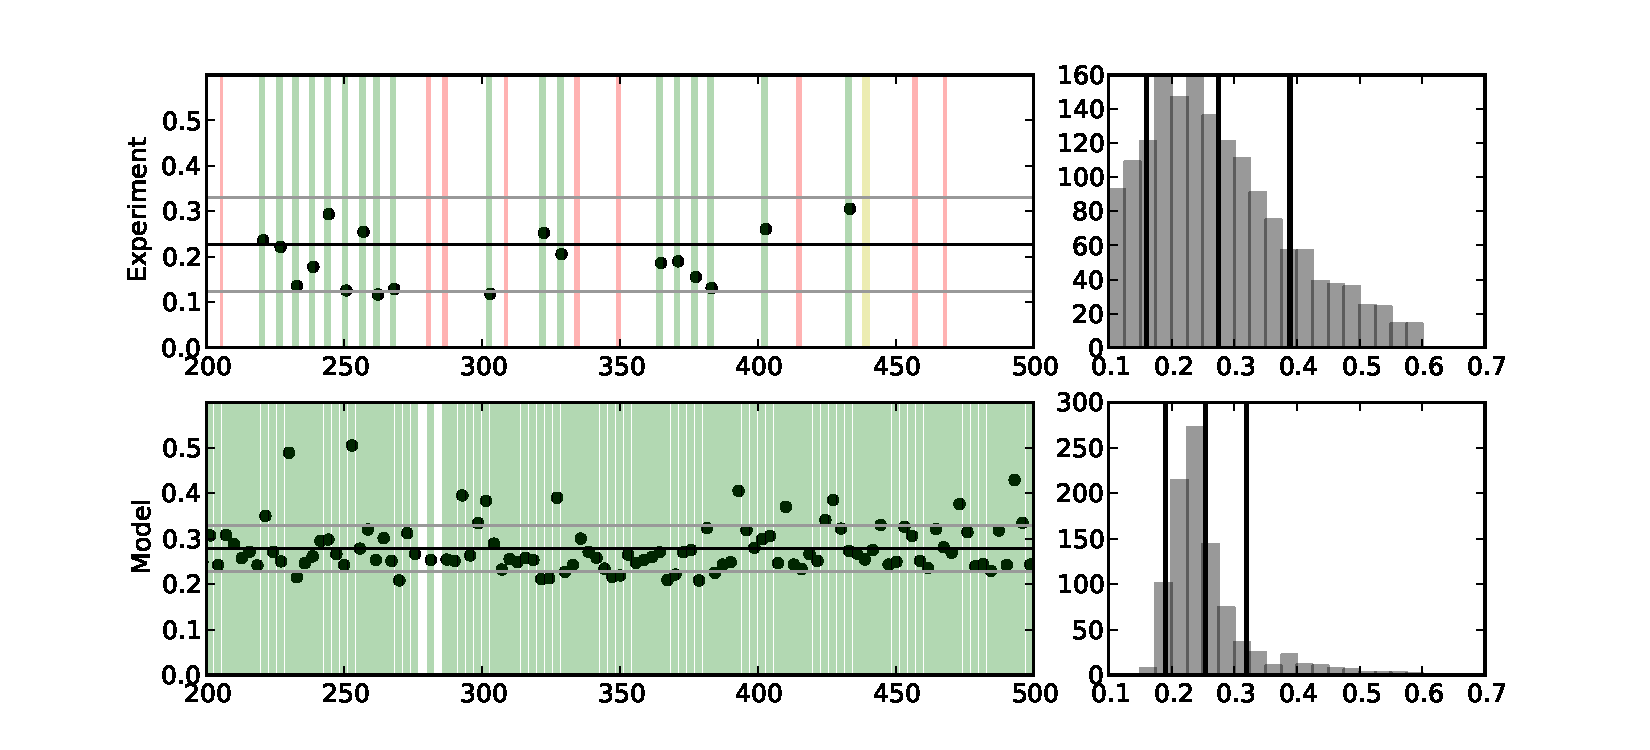
\includegraphics[width=\columnwidth]{f5-behaviour}
    \caption{Summary of model and experimental behaviour.
      (Left) Seconds 200 - 500 of an experimental (top)
      and model (bottom) session.
      (Right) Histograms of reactions times for
      experimental and model subjects.}
\end{figure}

\clearpage

\begin{figure}
  \centering
    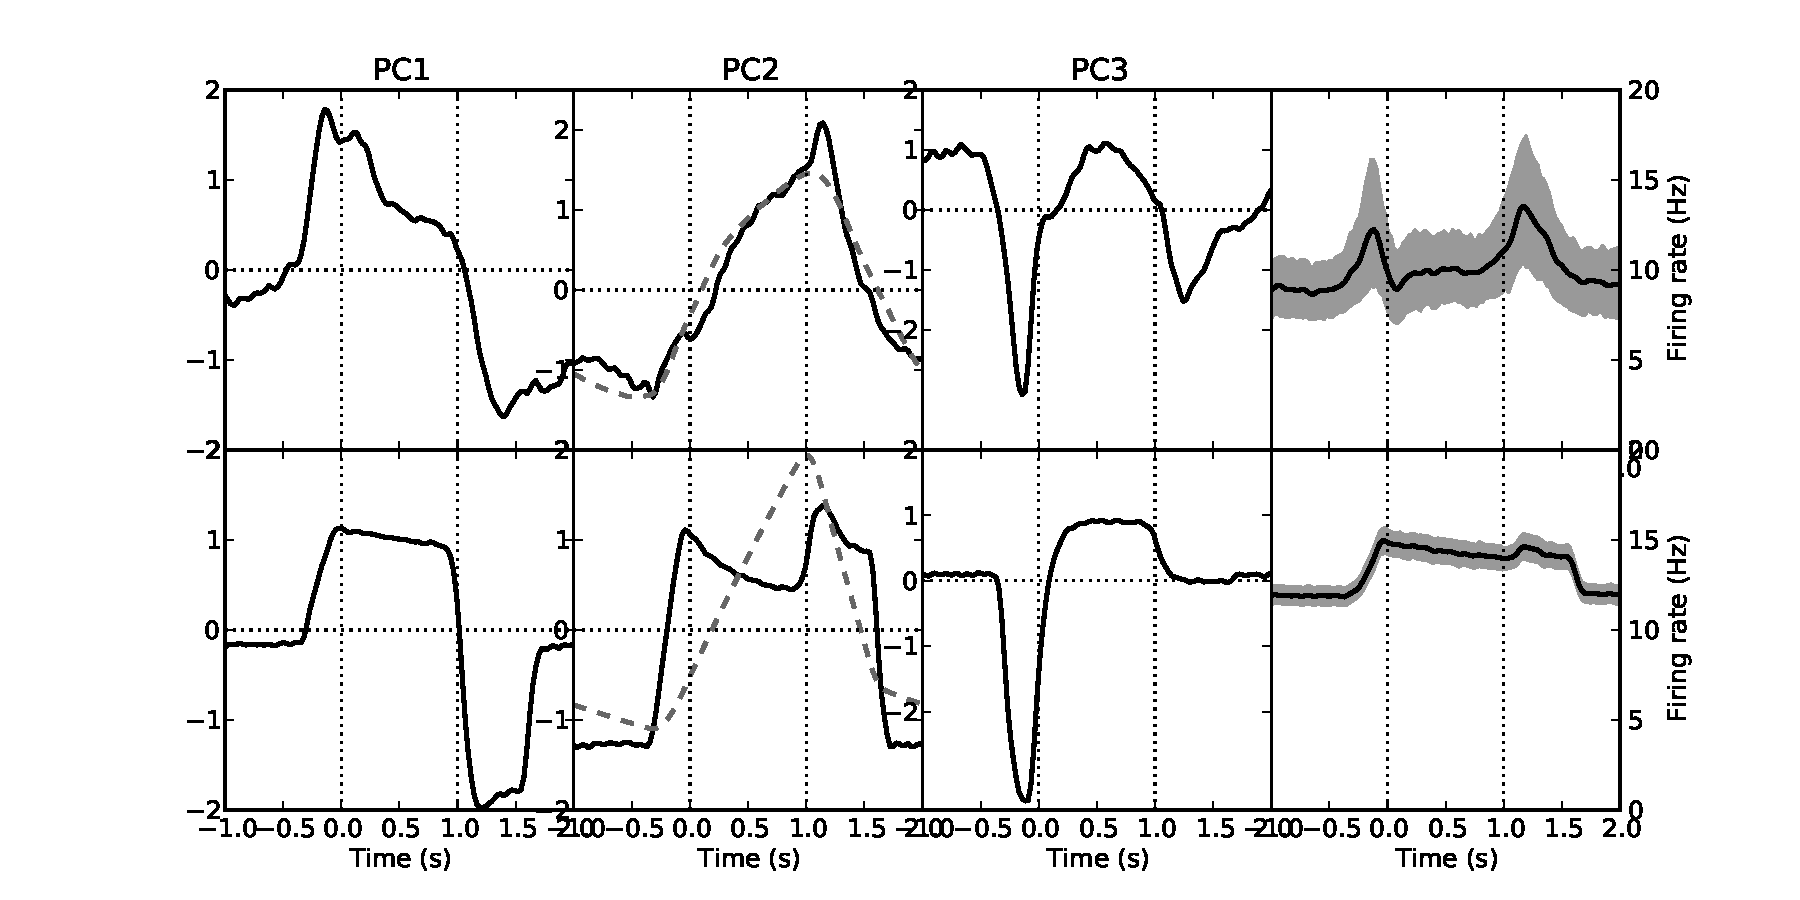
\includegraphics[width=\columnwidth]{f6-mcpca}
    \caption{Principal components identified in motor cortex
      spike data. (Top) Experiment. (Bottom) Model.}
\end{figure}

\clearpage

\begin{figure}
  \centering
    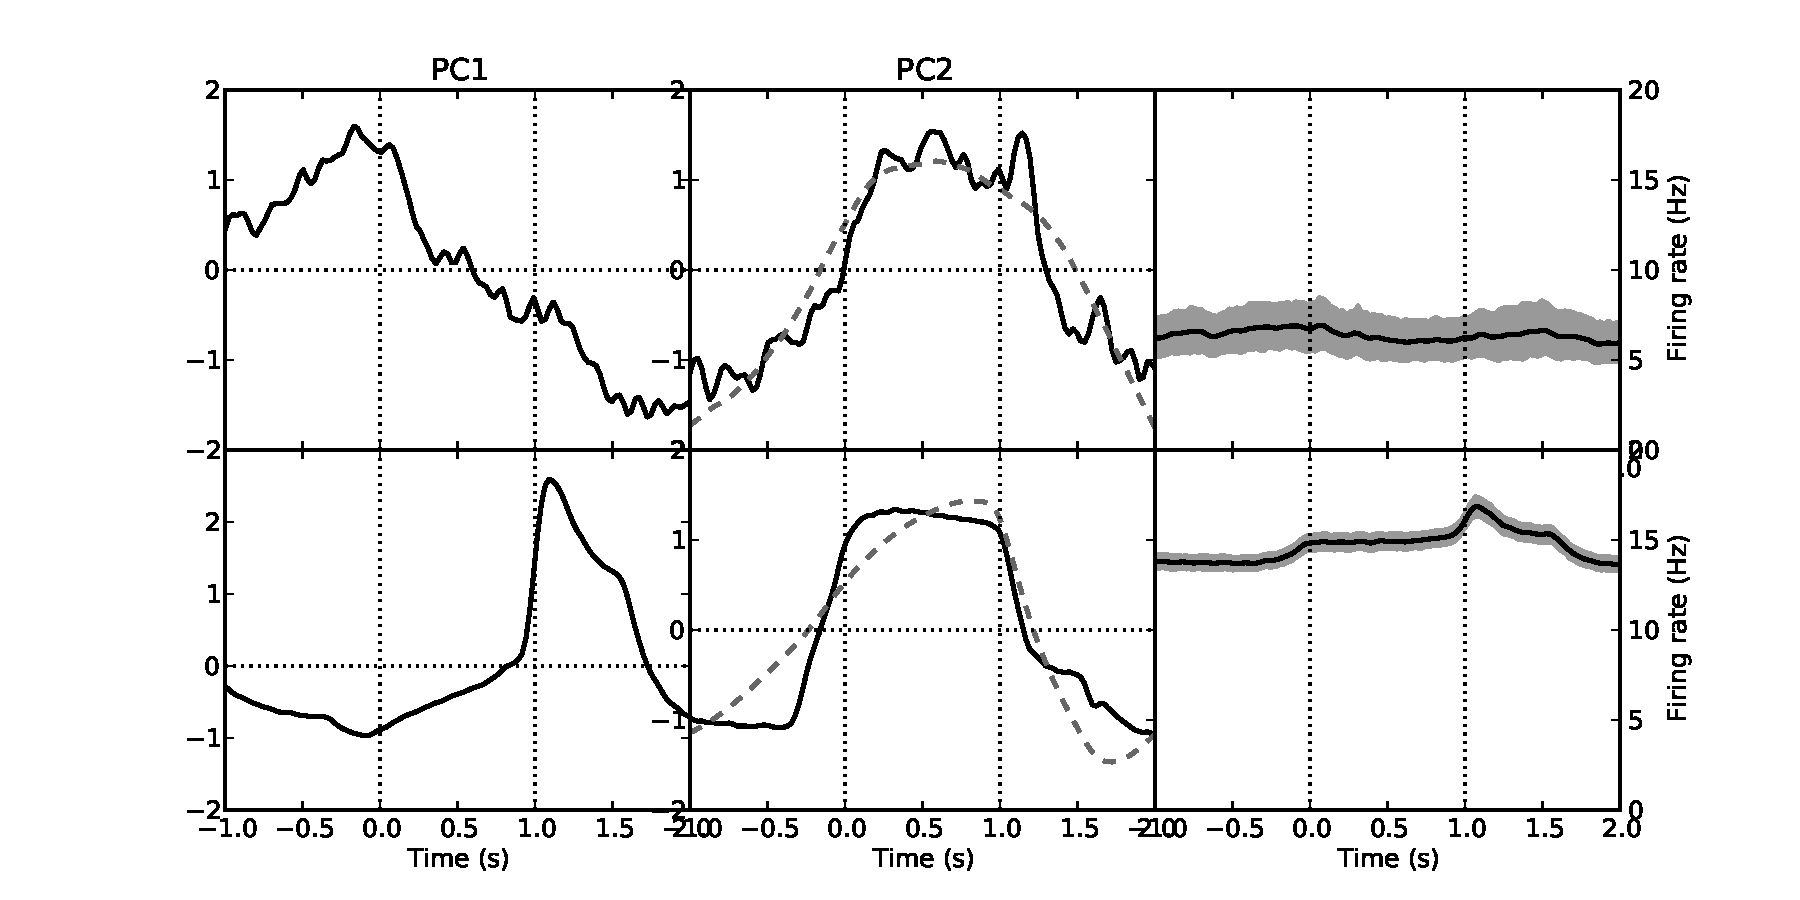
\includegraphics[width=\columnwidth]{f7-pfcpca}
    \caption{Principal components identified in medial prefrontal
      cortex spike data. (Top) Experiment. (Bottom) Model.}
\end{figure}

\clearpage

\begin{figure}
  \centering
    % 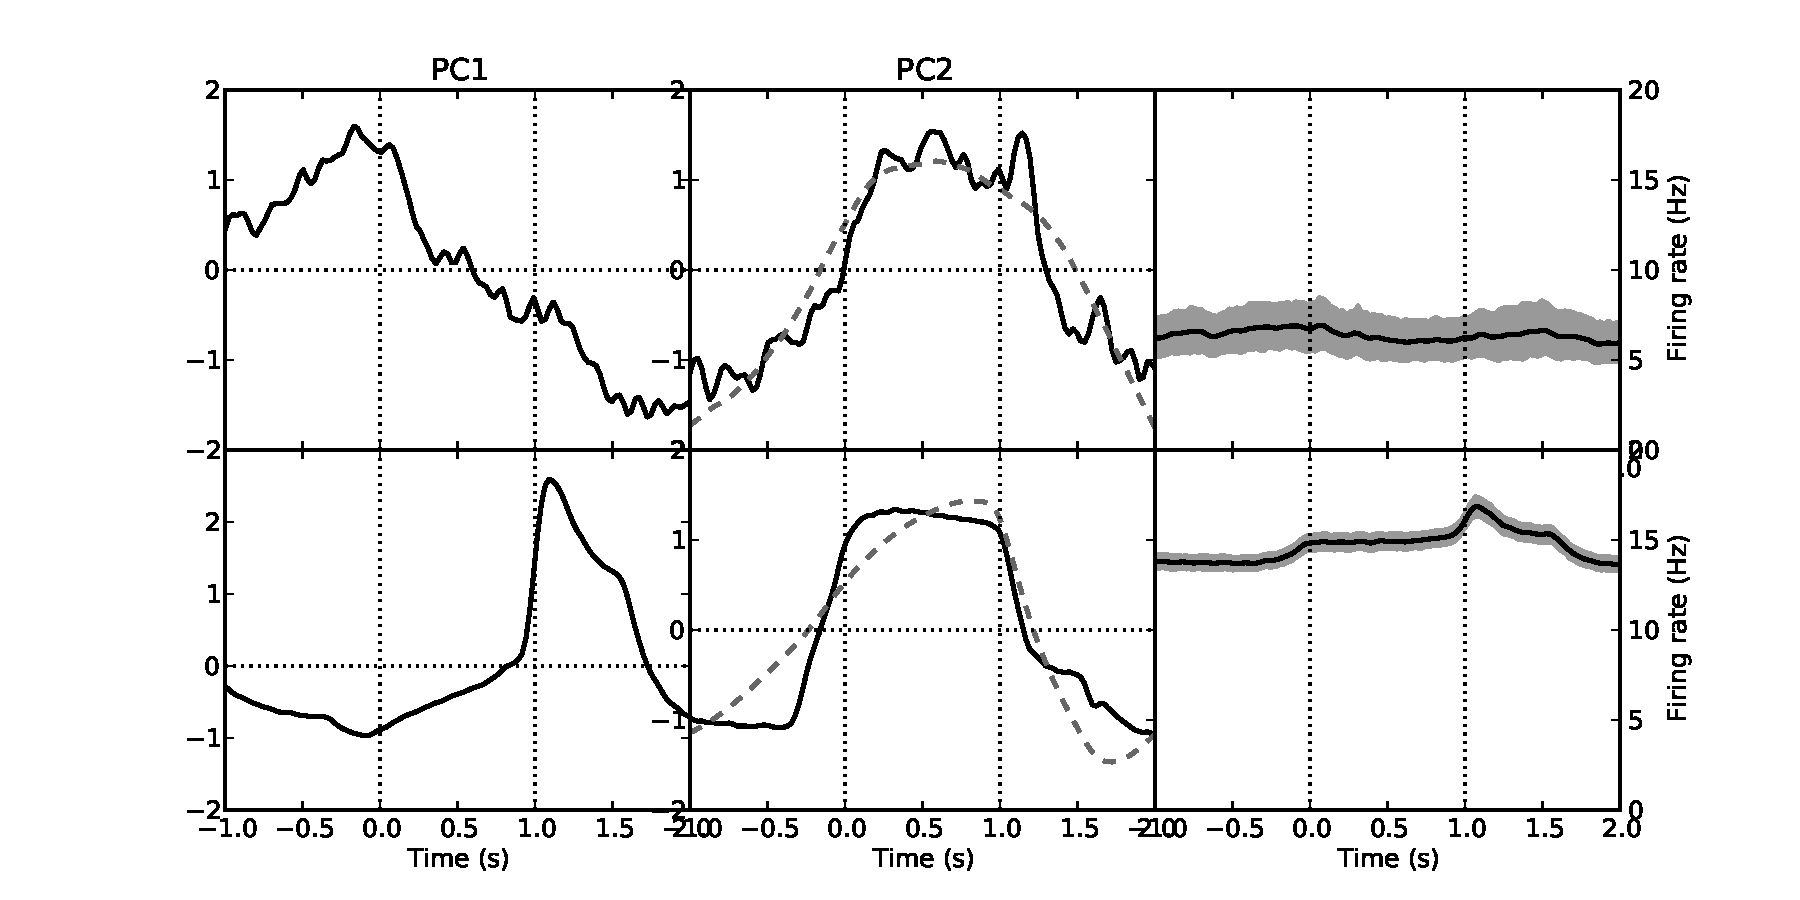
\includegraphics[width=\columnwidth]{f7-pfcpca}
    Placeholder
    \caption{Aging results}
\end{figure}

\clearpage

\begin{figure}
  \centering
    % 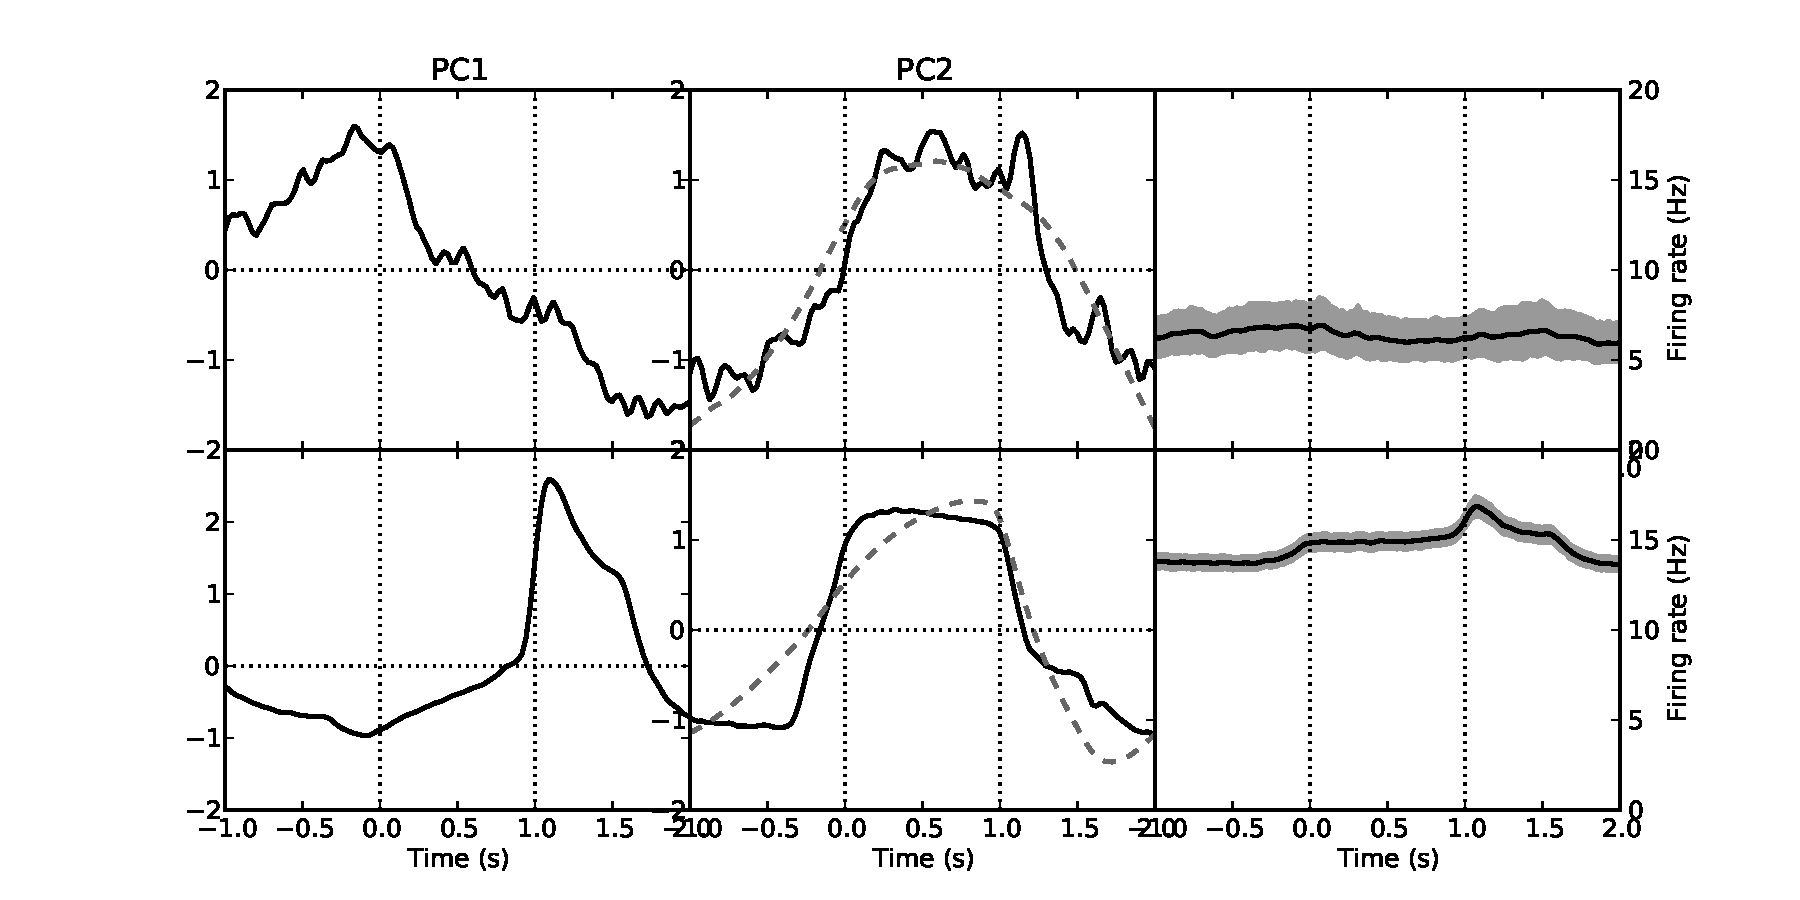
\includegraphics[width=\columnwidth]{f7-pfcpca}
    Placeholder
    \caption{Lesion results}
\end{figure}

\clearpage

\begin{figure}
  \centering
    % 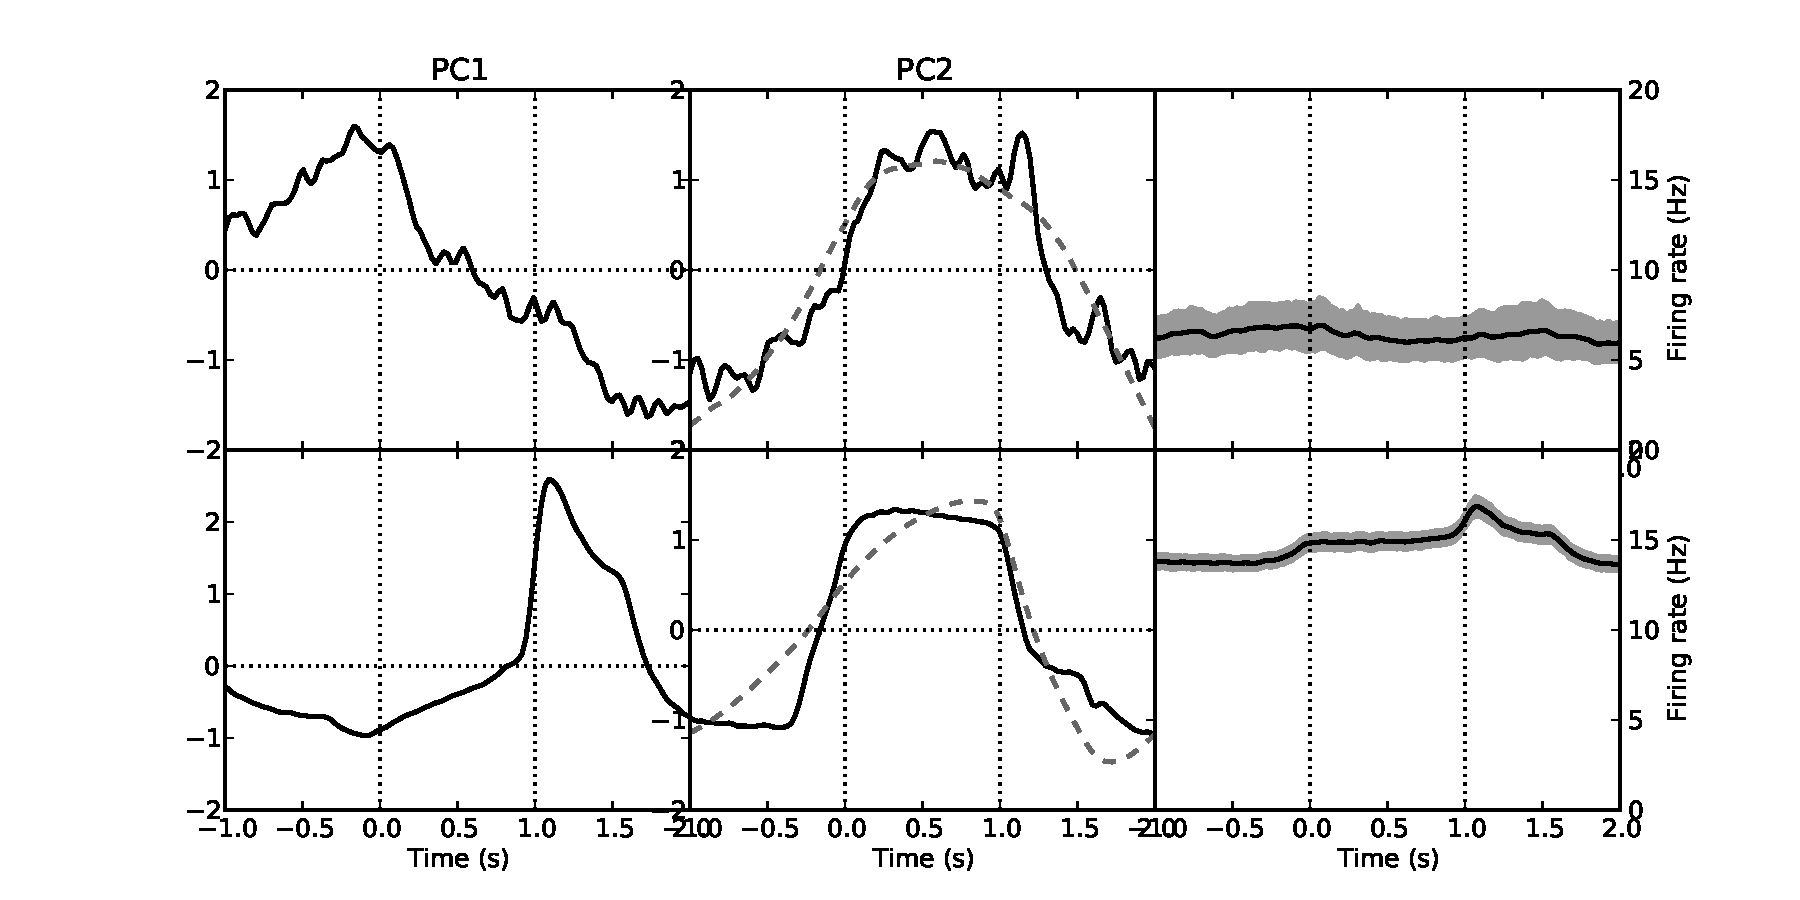
\includegraphics[width=\columnwidth]{f7-pfcpca}
    Placeholder
    \caption{Cooling results}
\end{figure}

\end{document}
